%%%%%%%%%%%%%%%%%%%%%%%%%%%%%%%%%%%%%%%%%
% University/School Laboratory Report
% LaTeX Template
% Version 3.1 (25/3/14)
%
% This template has been downloaded from:
% http://www.LaTeXTemplates.com
%
% Original author:
% Linux and Unix Users Group at Virginia Tech Wiki 
% (https://vtluug.org/wiki/Example_LaTeX_chem_lab_report)
%
% License:
% CC BY-NC-SA 3.0 (http://creativecommons.org/licenses/by-nc-sa/3.0/)
%
%%%%%%%%%%%%%%%%%%%%%%%%%%%%%%%%%%%%%%%%%

%----------------------------------------------------------------------------------------
%	PACKAGES AND DOCUMENT CONFIGURATIONS
%----------------------------------------------------------------------------------------

\documentclass[UTF8]{article}

\usepackage[version=3]{mhchem} % Package for chemical equation typesetting
\usepackage{siunitx} % Provides the \SI{}{} and \si{} command for typesetting SI units
\usepackage{graphicx} % Required for the inclusion of images
\usepackage{natbib} % Required to change bibliography style to APA
\usepackage{amsmath} % Required for some math elements 
\usepackage{ctex}
\usepackage{listings}
\usepackage{xcolor}
\usepackage{multirow}
\usepackage{url}
\setlength\parindent{0pt} % Removes all indentation from paragraphs

\renewcommand{\labelenumi}{\alph{enumi}.} % Make numbering in the enumerate environment by letter rather than number (e.g. section 6)

%\usepackage{times} % Uncomment to use the Times New Roman font

%----------------------------------------------------------------------------------------
%	DOCUMENT INFORMATION
%----------------------------------------------------------------------------------------

\title{\textbf{Introduction to High Performance Computing} \\ \textbf{PA1} \\ \textbf{Report}} % Title

\author{计86 \quad 任一\quad 2018011423} % Author name

\date{\today} % Date for the report


\lstset{
    % backgroundcolor=\color{red!50!green!50!blue!50},%代码块背景色为浅灰色
    rulesepcolor= \color{gray}, %代码块边框颜色
    % breaklines=true,  %代码过长则换行
    numbers=left, %行号在左侧显示
    numberstyle= \small,%行号字体
    keywordstyle= \color{blue},%关键字颜色
    commentstyle=\color{gray}, %注释颜色
    frame=shadowbox%用方框框住代码块
}
\begin{document}

\maketitle % Insert the title, author and date


\begin{center}
    \begin{tabular}{l  r}
    \hline

        \multicolumn{2}{c}{实验环境} \\ \hline
        操作系统: & Windows10家庭版 18362.72 Windows Subsystem for Linux \\ \hline% Date the experiment was performed
        mpicc版本: & gcc version 7.5.0 \\ \hline% Partner names


    \end{tabular}
\end{center}


\newpage

%----------------------------------------------------------------------------------------
%	SECTION 1
%----------------------------------------------------------------------------------------

\section{Ex3.13}
\subsection{解题思路}
本题主要任务是解决MPI\_Scatter和MPI\_Gather在数组长度无法被进程数整除时不能使用的问题,
因此在本题中,我使用了MPI\_Scatterv和MPI\_Gatherv进行数组的分发和收集。\\


在MPI\_Scatterv和MPI\_Gatherv这两个函数中,与MPI\_Scatter和MPI\_Gather较为不同的两个参数是displacement和datacount,这两个参数都是整型数组类型的。
displacement指各进程接收到的数据在数组中的开始位置,datacount则是每个进程所接收的数据量,通过这两个参数的指定,MPI\_Scatterv和MPI\_Gatherv即可
实现每个进程分配指定数量的数据,因而更为灵活一些。 \\


由于第一次书面作业的Exercise1.1中涉及到了此题的理论基础,即在数组长度不能被进程数整除时,各进程的元素分配计算,因此只需参考第一次作业Exercise1.1题的结果,即可完成此题中displacement和datacount参数的计算。
不过还有一种特殊情况是,数组长度小于进程数。我对于这种情况的处理是,优先进程编号小的进程获得数据,即进程编号小于数组长度的进程分配一个元素,其他进程不分配元素也不参与运算。
但是涉及到其他无元素进程的内存分配问题还值得商榷,例如出现malloc(0)这样的情况,这种情况的可靠性还有待商榷,不过在本实验的测试中,这种方法并没有问题。

\subsection{测试}
本并行程序的测试通过与串行程序的对拍进行。在本地测试中,对拍1000组数据没有产生错误。
下面是部分对拍测试截图。在集群上,只需在本题文件夹下输入make run命令即可运行本程序(makefile中设置了默认使用4进程),输入make check命令即可进行对拍测试,更多测试功能详见本题makefile.

\begin{figure}[h]
    \centering
    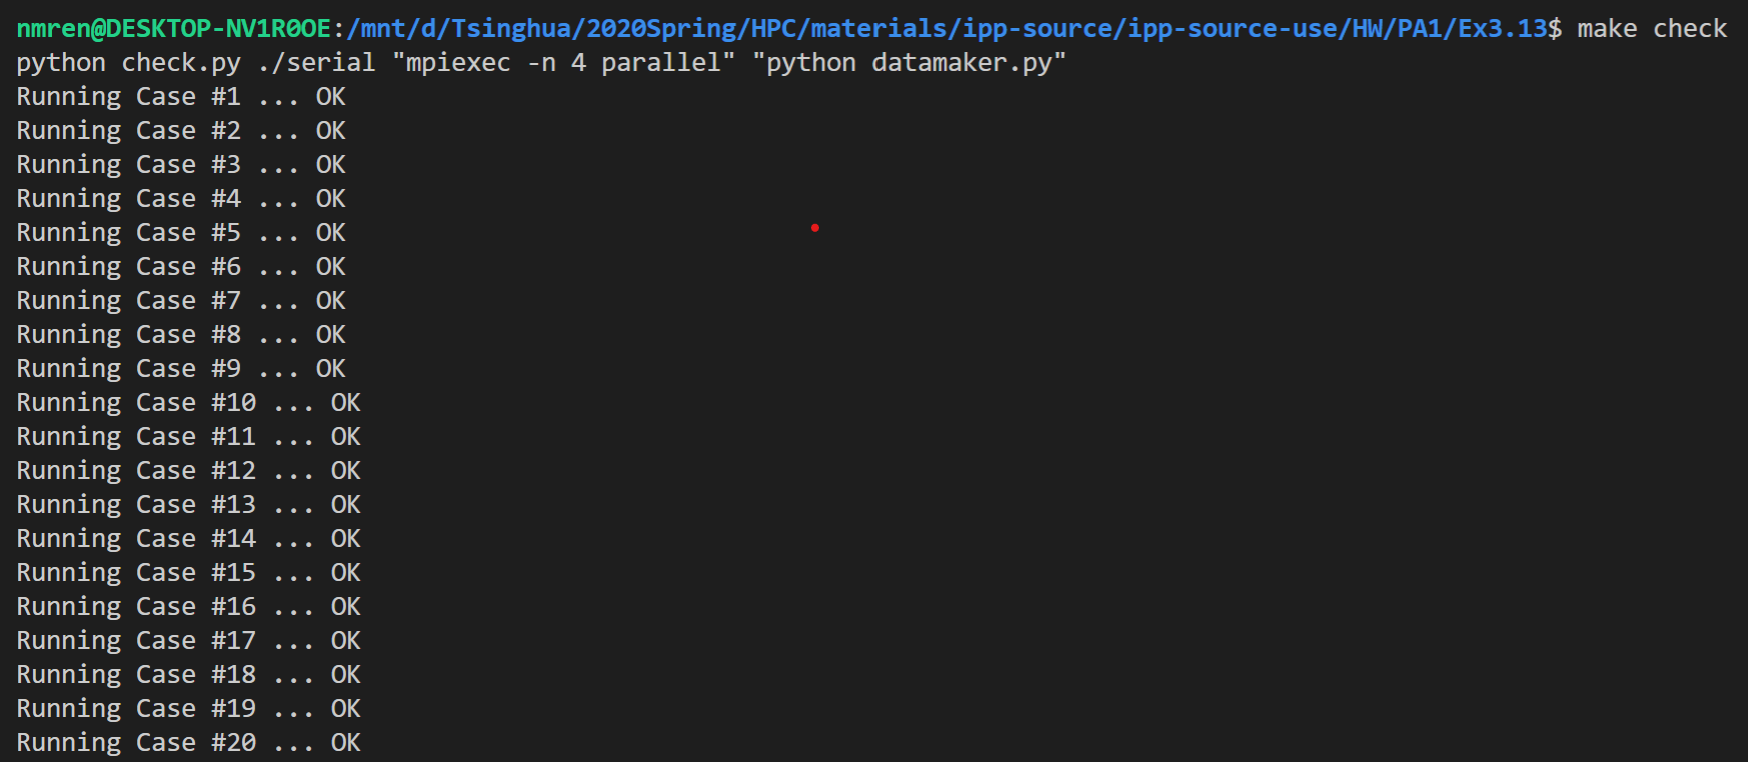
\includegraphics[width=\textwidth]{checkResult.png}
    \caption{并行程序与对拍程序部分结果图}
\end{figure}

\begin{figure}[h]
    \centering
    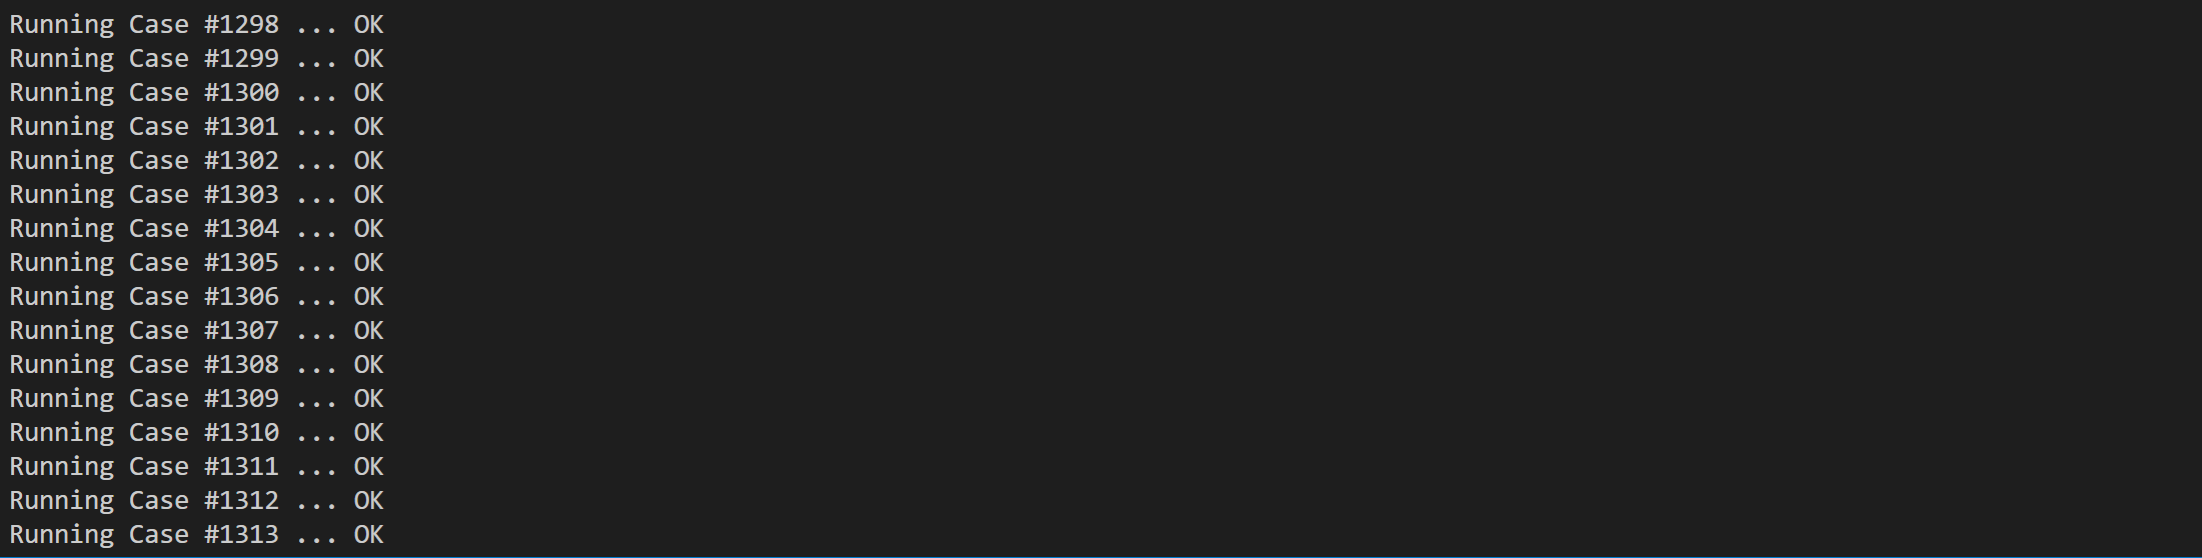
\includegraphics[width=\textwidth]{checkResult1.png}
    \caption{并行程序与对拍程序部分结果图}
\end{figure}


\clearpage

 
%----------------------------------------------------------------------------------------
%	SECTION 2
%----------------------------------------------------------------------------------------

\section{Exercise 3.11}
\subsection{解题思路}
本题使用MPI\_Scan函数,对p个进程,每个进程有10个元素的数组求了前缀和。我的思路是,
首先对每个进程求局部和,然后利用MPI\_Scan函数,
使得每个进程i都有进程0至i这i+1个进程的元素总和,接着在每个进程里,通过用MPI\_Scan
得到的总和,从后向前累计减去当前进程中的元素,即可所求的全局前缀和。
最后将这些全局前缀和通过MPI\_Gather函数,汇总到0号进程统一输出。

\subsection{测试}
为了测试,我编写了串行求前缀和的程序,
与并行程序进行对拍。通过本机测试得到,对拍1000组长度为40的前缀求和,没有发生错误。

\subsection{运行方式}
为了能够满足题目中"每个进程随机生成的10个数"以及与串行程序对拍的需求,我参考了ch3中mpi\_odd\_even.c中
实现的命令行参数控制数据输入方式。\\\\

具体来说,在集群上运行srun -n <p> parallel -<g|i>, 其中p代表进程数,-g代表使用自动随机生成的数据,-i代表使用用户从命令行输入的10p个数据。通过-i的命令设置,
我能够从文件中重定向输入,从而完成与串行程序的对拍。在集群上,只需在本题文件夹下输入make run命令即可运行本程序(makefile中设置了默认使用4进程),输入make check命令即可进行对拍测试,更多测试功能详见本题makefile.
\clearpage
\section{Ex 3.1}
\subsection{解题思路}
本题需要补充Find\_bins和Which\_bins函数。在Find\_bins函数中,通过调用Which\_bins函数统计当前进程所负责的元素在
哪个bin中,得到局部的bin计数之后,使用MPI\_Reduce函数将结果快速求和到0号进程。\\\\
在Which\_bins函数中,由于每个bin的宽度都已知,是$bin\_maxes[0] - min\_meas$, 因此$data$所在的bin编号即为$(int)((data - min\_meas) / (bin\_maxes[0] - min\_meas))$
\subsection{测试}
本程序在本地与集群上测试均表现正常。在集群上,只需在本题文件夹下输入make run命令即可运行本程序(makefile中设置了默认使用4进程).
\clearpage
\section{Ex3.5}
\subsection{解题思路}
在本题中,我使用了附上的prog3.5\_mpi\_mat\_vect\_col.c程序完成。在这份代码中,已经基本实现了0号进程并行按列分块然后分发到不同进程的功能。
其中关键的函数是Build\_derived\_type中的MPI\_Type\_vector和MPI\_Type\_create\_resized. 
\\\\
MPI\_Type\_vector接受5个参数,前三个较为关键,
分别是Number of blocks, Number of elements in blocks, Number of elements between start of each block.
 \footnote{此处参考\url{https://www.open-mpi.org/doc/current/man3/MPI_Type_vector.3.php}} 
如果设矩阵是$m*n$阶,进程数是$comm\_sz$,那么这三个参数分别应该设为$m, n/comm\_sz, n$,这样就可以满足
把待计算的矩阵根据进程数按列分块,每个进程得到$m * (n/comm\_sz)$阶的矩阵进行计算。最后再使用MPI\_Reduce得到最终结果。
而MPI\_Type\_create\_resized共接收4个参数,本题中较为关键的是第2个参数和第3个参数,含义分别为New lower bound of data type, New extent of data type. 
\footnote{此处参考\url{https://www.open-mpi.org/doc/current/man3/MPI_Type_create_resized.3.php}}
这两个参数在本题中分别设置为$0, n/comm\_sz$. 这样可以理解为,把新生成的数据类型的宽度调整为$n/comm\_sz$,这样就可以在本题中方便地实现Scatter.
\\\\

下图示意了本题如何按列分块。
\footnote{此图来源\url{https://pdfs.semanticscholar.org/afa8/9673d416faf99cfd6b4353ab810e8418f5d7.pdf}}
\begin{figure}[h]
    \centering
    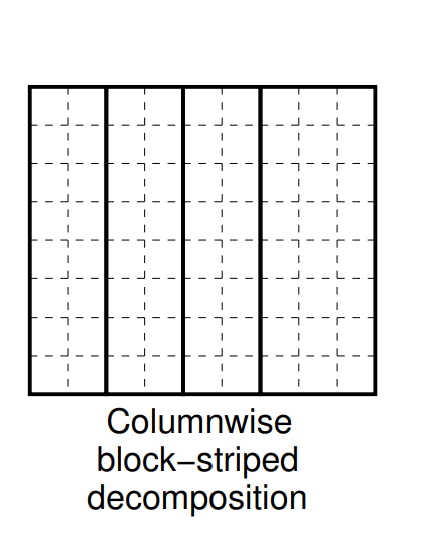
\includegraphics[width=0.2\textwidth]{cw.png}
    \caption{通过MPI\_Type\_vector和MPI\_Type\_create\_resized实现矩阵按列分块读取}
\end{figure}
\subsection{运行方式}
在集群上,只需在本题文件夹下输入make run命令即可运行本程序(makefile中设置了默认使用4进程),在运行make run后输入python check.py即可自动测试本报告中的数据,并且重定向到result文件夹下进行输出。
\clearpage
\subsection{测试结果}
本题进行的所有测试,并行计算结果与串行计算结果均相同(差的二范数为0),从而保证了并行程序的正确性。
\subsubsection{并行计算时间和串行计算时间图表分析}


\begin{table}[h]
    \caption{Ex3.5 并行计算时间(s)}
    \label{tab:my-table}
    \centering
    \scalebox{0.8} {
    \begin{tabular}{|c|c|c|c|c|c|c|c|}
    \hline
                                & \multicolumn{7}{c|}{Matrix Order}                                    \\ \hline
    \multirow{7}{*}{Processors} &    & 1024     & 2048     & 4096     & 8192     & 16384    & 32768    \\ \cline{2-8} 
                                & 1  & 0.006984 & 0.018833 & 0.051525 & 0.232303 & 0.82091  & 3.714691 \\ \cline{2-8} 
                                & 2  & 0.003527 & 0.009607 & 0.025758 & 0.116467 & 0.410803 & 1.863362 \\ \cline{2-8} 
                                & 4  & 0.001778 & 0.004934 & 0.014211 & 0.056639 & 0.233671 & 0.873432 \\ \cline{2-8} 
                                & 8  & 0.000901 & 0.002473 & 0.007457 & 0.029537 & 0.117692 & 0.470057 \\ \cline{2-8} 
                                & 16 & 0.00047  & 0.001307 & 0.003816 & 0.014908 & 0.059785 & 0.236177 \\ \cline{2-8} 
                                & 32 & 0.000258 & 0.000531 & 0.002265 & 0.008542 & 0.033146 & 0.120416 \\ \hline
    \end{tabular}}
    \end{table}



% Please add the following required packages to your document preamble:
% \usepackage{multirow}
\begin{table}[h]
    \caption{Ex3.5 串行计算时间(s)}
    \label{tab:my-table}
    \centering
    \scalebox{0.8} {
    \begin{tabular}{|c|c|c|c|c|c|c|c|}
    \hline
                                & \multicolumn{7}{c|}{Matrix Order}                                    \\ \hline
    \multirow{7}{*}{Processors} &    & 1024     & 2048     & 4096     & 8192     & 16384    & 32768    \\ \cline{2-8} 
                                & 1  & 0.006748 & 0.017442 & 0.051249 & 0.262236 & 0.819512 & 3.715776 \\ \cline{2-8} 
                                & 2  & 0.006644 & 0.018268 & 0.051153 & 0.232251 & 0.821548 & 3.714187 \\ \cline{2-8} 
                                & 4  & 0.006783 & 0.018551 & 0.056124 & 0.224963 & 0.931101 & 3.280052 \\ \cline{2-8} 
                                & 8  & 0.006998 & 0.018533 & 0.051223 & 0.232268 & 0.929077 & 3.715156 \\ \cline{2-8} 
                                & 16 & 0.006745 & 0.018167 & 0.058115 & 0.23203  & 0.901695 & 3.714686 \\ \cline{2-8} 
                                & 32 & 0.007508 & 0.014606 & 0.05868  & 0.234549 & 0.936246 & 4.624938 \\ \hline
    \end{tabular}}
    \end{table}

    \begin{figure}[h]
        \centering
        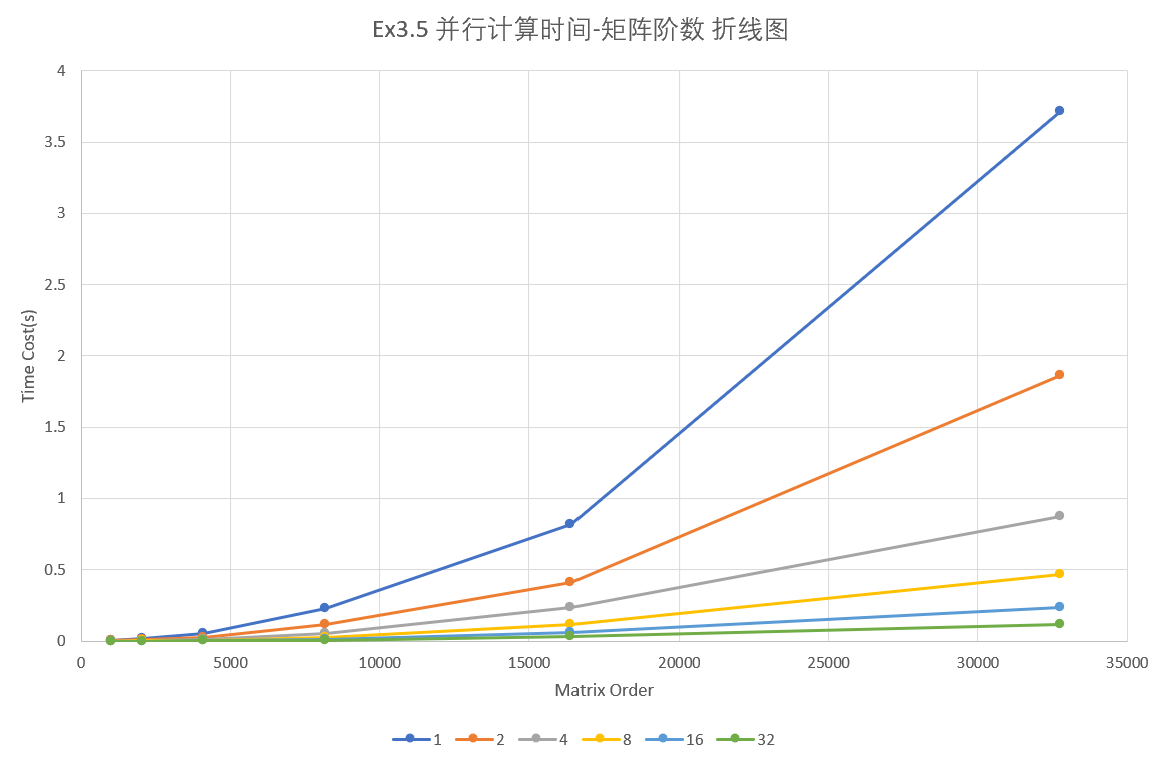
\includegraphics[width=0.85\textwidth]{35pto.png}
        \caption{Ex3.5 并行计算时间-矩阵阶数 折线图}
    \end{figure}

    \begin{figure}[h]
        \centering
        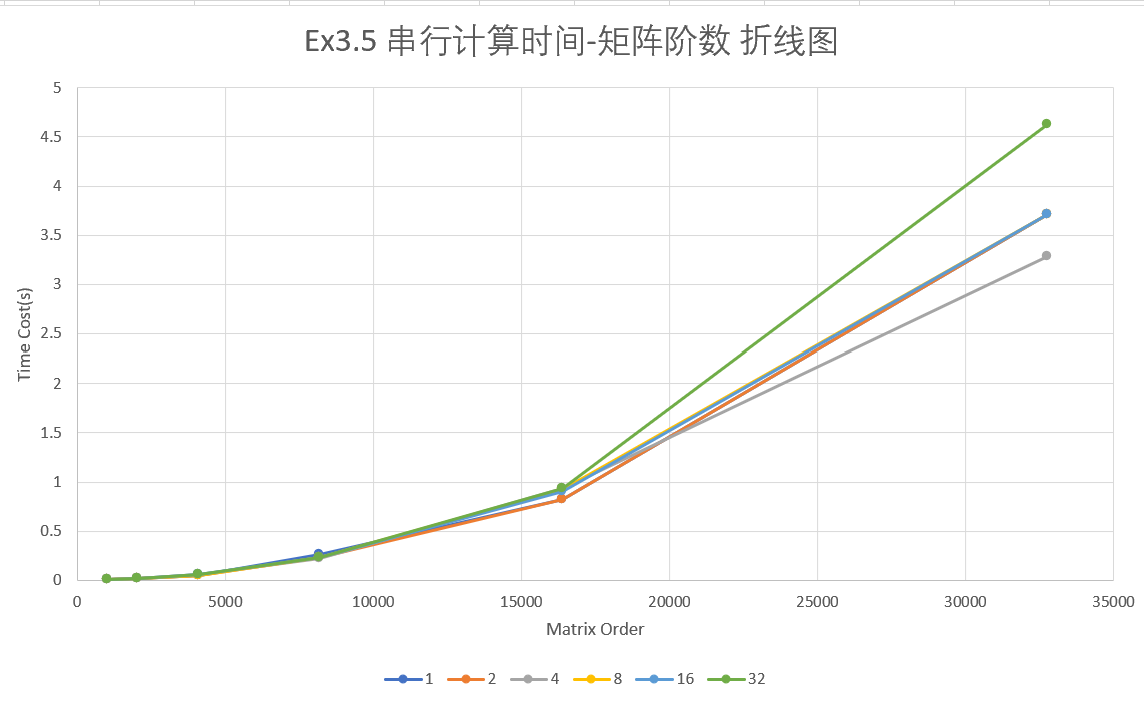
\includegraphics[width=0.85\textwidth]{35sto.png}
        \caption{Ex3.5 串行计算时间-矩阵阶数 折线图}
    \end{figure}
    本部分中展示了不同进程数下,并行和串行计算时间随着矩阵阶数的变化表格和折线图。
    从图4中可以清晰看出,并行计算时间与矩阵阶数成正相关。由于矩阵元素数量与矩阵阶数
    成二次关系,图中的耗时与矩阵阶数也可以近似看作二次关系。同时可以看出,进程数越多,并行计算时间越少,这也充分体现了
    并行计算在计算时的优越性。\\\\

    从图5中可以看出,串行计算时间与矩阵阶数近似为二次关系。不过矩阵阶数一定,不同的进程数下串行计算时间基本相同,这也基本符合串行计算
    在本实验中只由0号进程计算的事实。同时从图中和表格中都可以看到,在矩阵阶数一定时,并行计算的时间要远低于串行计算,这再一次表明了并行程序在计算方面的优越性。


\clearpage
\subsubsection{并行分配时间与总时间图表分析}

% Please add the following required packages to your document preamble:
% \usepackage{multirow}
\begin{table}[h]
    \caption{Ex3.5 并行分配时间(s)}
    \label{tab:my-table}
    \centering
    \scalebox{0.8} {
    \begin{tabular}{|c|c|c|c|c|c|c|c|}
    \hline
                                & \multicolumn{7}{c|}{Matrix Order}                                    \\ \hline
    \multirow{7}{*}{Processors} &    & 1024     & 2048     & 4096     & 8192     & 16384    & 32768    \\ \cline{2-8} 
                                & 1  & 0.003748 & 0.011979 & 0.040306 & 0.165983 & 0.65822  & 2.654574 \\ \cline{2-8} 
                                & 2  & 0.034063 & 0.106454 & 0.304867 & 1.104077 & 3.911728 & 16.8321  \\ \cline{2-8} 
                                & 4  & 0.034214 & 0.108905 & 0.315048 & 1.101445 & 4.37147  & 15.888   \\ \cline{2-8} 
                                & 8  & 0.03481  & 0.108111 & 0.29167  & 1.121542 & 4.309148 & 17.13832 \\ \cline{2-8} 
                                & 16 & 0.036225 & 0.106354 & 0.276049 & 1.11216  & 4.273796 & 17.19085 \\ \cline{2-8} 
                                & 32 & 0.115958 & 0.254139 & 6.009296 & 3.238718 & 95.0812  & 52.53218 \\ \hline
    \end{tabular}}
    \end{table}


% Please add the following required packages to your document preamble:
% \usepackage{multirow}
\begin{table}[h]
    \caption{Ex3.5 并行总时间(s)}
    \label{tab:my-table}
    \centering
    \scalebox{0.8} {
    \begin{tabular}{|c|c|c|c|c|c|c|c|}
    \hline
                                & \multicolumn{7}{c|}{Matrix Order}                                    \\ \hline
    \multirow{7}{*}{Processors} &    & 1024     & 2048     & 4096     & 8192     & 16384    & 32768    \\ \cline{2-8} 
                                & 1  & 0.010732 & 0.030812 & 0.091831 & 0.398286 & 1.47913  & 6.369265 \\ \cline{2-8} 
                                & 2  & 0.03759  & 0.116061 & 0.330625 & 1.220544 & 4.322531 & 18.69546 \\ \cline{2-8} 
                                & 4  & 0.035992 & 0.113839 & 0.329259 & 1.158084 & 4.605141 & 16.76143 \\ \cline{2-8} 
                                & 8  & 0.035711 & 0.110584 & 0.299127 & 1.151079 & 4.42684  & 17.60837 \\ \cline{2-8} 
                                & 16 & 0.036695 & 0.107661 & 0.279865 & 1.127068 & 4.333581 & 17.42703 \\ \cline{2-8} 
                                & 32 & 0.116216 & 0.25467  & 6.011561 & 3.24726  & 95.11434 & 52.6526  \\ \hline
    \end{tabular}}
    \end{table}


    \begin{figure}[h]
        \centering
        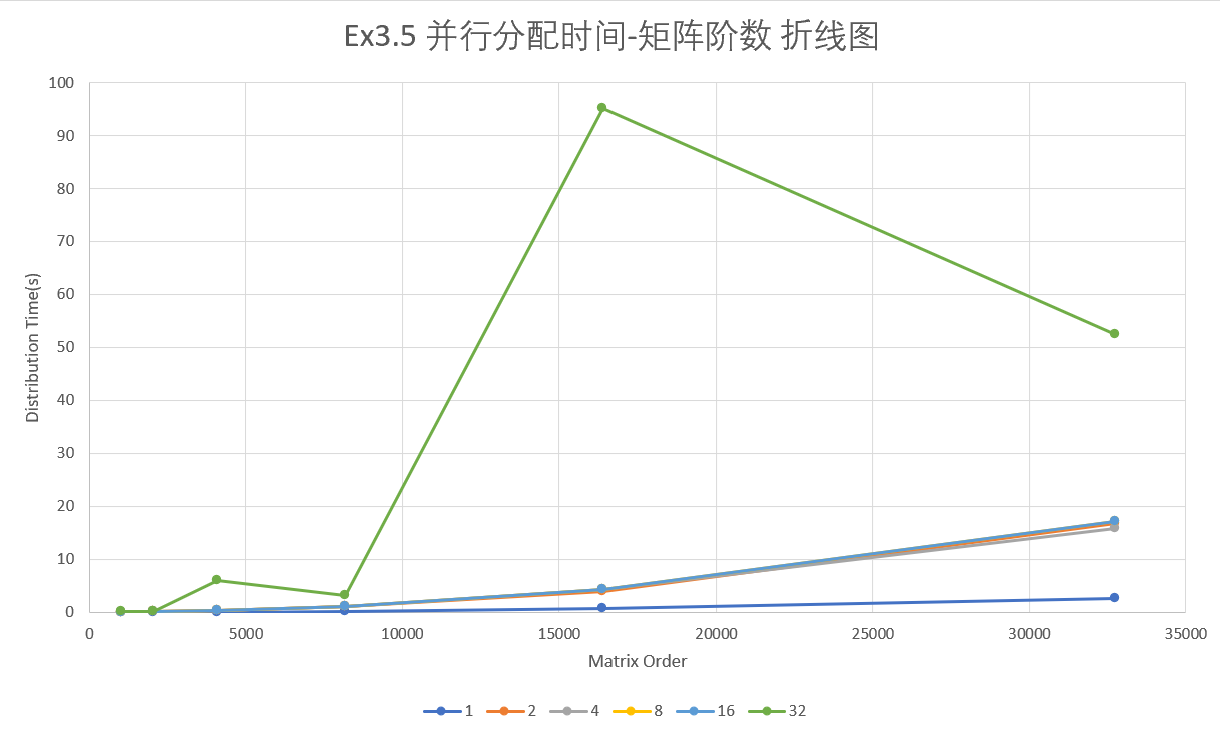
\includegraphics[width=0.85\textwidth]{35pdo.png}
        \caption{Ex3.5 并行分配时间-矩阵阶数 折线图}
    \end{figure}

    \begin{figure}[h]
        \centering
        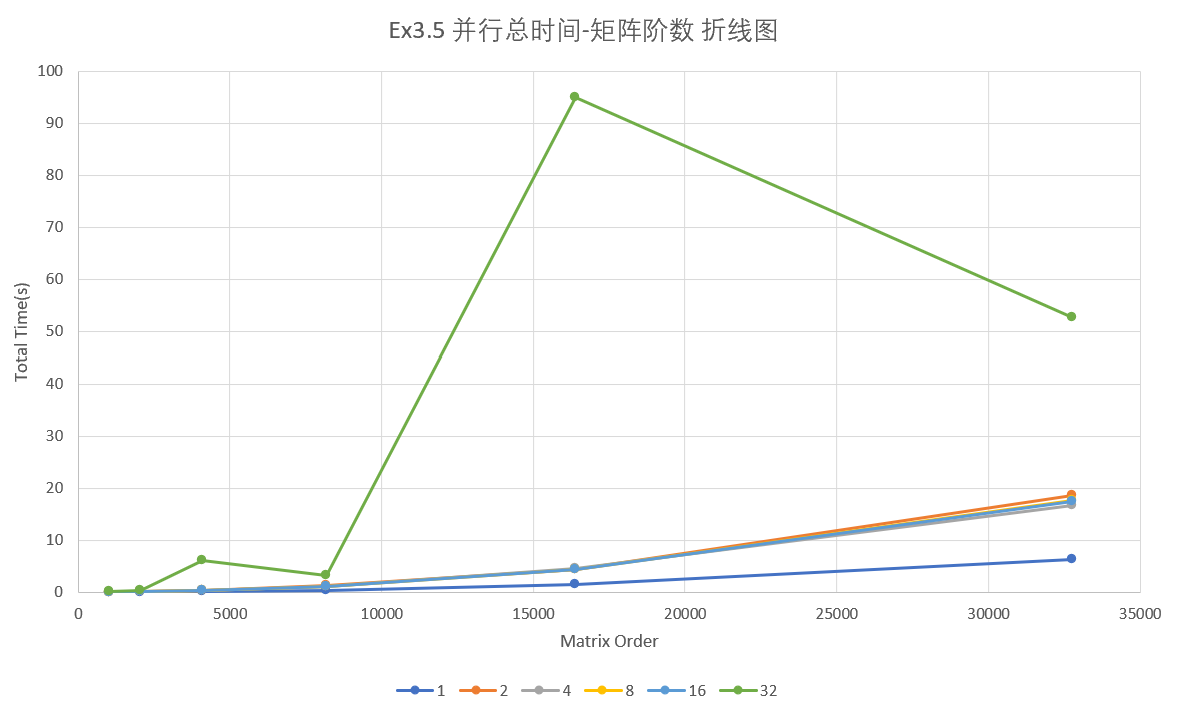
\includegraphics[width=0.85\textwidth]{35ptto.png}
        \caption{Ex3.5 并行总时间-矩阵阶数 折线图}
    \end{figure}
    本部分展示了不同进程数下,并行分配时间和并行计算总时间与矩阵阶数的关系图表。
    从图6中可以看出,并行分配时间与矩阵阶数成正相关关系,不考虑进程数为32的图线的情况下,
    并行分配时间仍可近似认为与矩阵阶数成二次关系。\\\\

    但是进程数为32时,当矩阵阶数是16384时,分配时间达到了95s,这个结果较为反常。
    于是我对这组数据又进行了几次测试,包括对结果正确性的检验。在额外的这几次测试中,我得到的并行分配时间和并行计算时间均在13-14s左右,符合图线趋势,也和串行计算的结果完全相同。
    于是我认为,图表中出现的这组异常数据,并非由于我的程序错误导致,而是OS状态等原因造成的偶然情况。

\clearpage
\subsubsection{并行计算时间加速比与并行总时间加速比}

% Please add the following required packages to your document preamble:
% \usepackage{multirow}
\begin{table}[h]
    \caption{Ex3.5 并行计算时间加速比}
    \label{tab:my-table}
    \centering
    \scalebox{0.8} {
    \begin{tabular}{|c|c|c|c|c|c|c|c|}
    \hline
                                & \multicolumn{7}{c|}{Matrix Order}                                    \\ \hline
    \multirow{7}{*}{Processors} &    & 1024     & 2048     & 4096     & 8192     & 16384    & 32768    \\ \cline{2-8} 
                                & 1  & 0.966208 & 0.92614  & 0.994643 & 1.128853 & 0.998297 & 1.000292 \\ \cline{2-8} 
                                & 2  & 1.883754 & 1.90153  & 1.985907 & 1.994136 & 1.999859 & 1.993272 \\ \cline{2-8} 
                                & 4  & 3.814961 & 3.75983  & 3.949335 & 3.971875 & 3.984666 & 3.75536  \\ \cline{2-8} 
                                & 8  & 7.766926 & 7.494137 & 6.869116 & 7.863629 & 7.894139 & 7.903629 \\ \cline{2-8} 
                                & 16 & 14.35106 & 13.89977 & 15.2293  & 15.56413 & 15.08229 & 15.7284  \\ \cline{2-8} 
                                & 32 & 29.10078 & 27.50659 & 25.90728 & 27.45832 & 28.24612 & 38.408   \\ \hline
    \end{tabular}}
    \end{table}

    % Please add the following required packages to your document preamble:
% \usepackage{multirow}
\begin{table}[h]
    \caption{Ex3.5 并行总时间加速比}
    \label{tab:my-table}
    \centering
    \scalebox{0.8} {
    \begin{tabular}{|c|c|c|c|c|c|c|c|}
    \hline
                                & \multicolumn{7}{c|}{Matrix Order}                                    \\ \hline
    \multirow{7}{*}{Processors} &    & 1024     & 2048     & 4096     & 8192     & 16384    & 32768    \\ \cline{2-8} 
                                & 1  & 0.628774 & 0.566078 & 0.55808  & 0.658411 & 0.55405  & 0.583392 \\ \cline{2-8} 
                                & 2  & 0.176749 & 0.1574   & 0.154716 & 0.190285 & 0.190062 & 0.198668 \\ \cline{2-8} 
                                & 4  & 0.188459 & 0.162958 & 0.170455 & 0.194254 & 0.202187 & 0.19569  \\ \cline{2-8} 
                                & 8  & 0.195962 & 0.167592 & 0.171242 & 0.201783 & 0.209874 & 0.210988 \\ \cline{2-8} 
                                & 16 & 0.183813 & 0.168743 & 0.207654 & 0.20587  & 0.208072 & 0.213157 \\ \cline{2-8} 
                                & 32 & 0.064604 & 0.057353 & 0.009761 & 0.07223  & 0.009843 & 0.087839 \\ \hline
    \end{tabular}}
    \end{table}


    \begin{figure}[h]
    \centering
        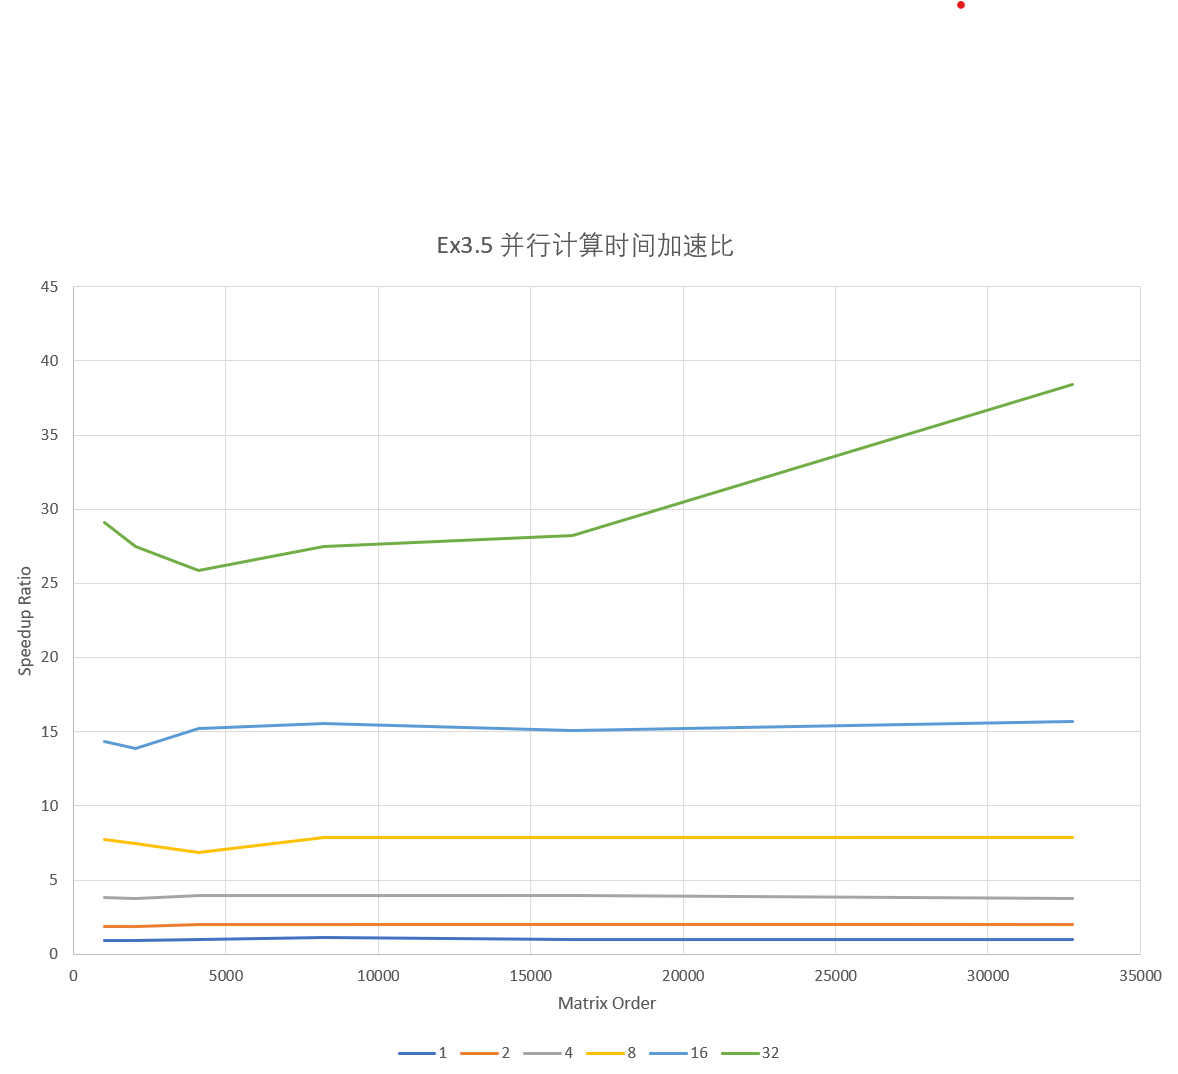
\includegraphics[width=0.85\textwidth]{35pct.png}
        \caption{Ex3.5 并行计算时间加速比}
    \end{figure}
    \begin{figure}[h]
    \centering
        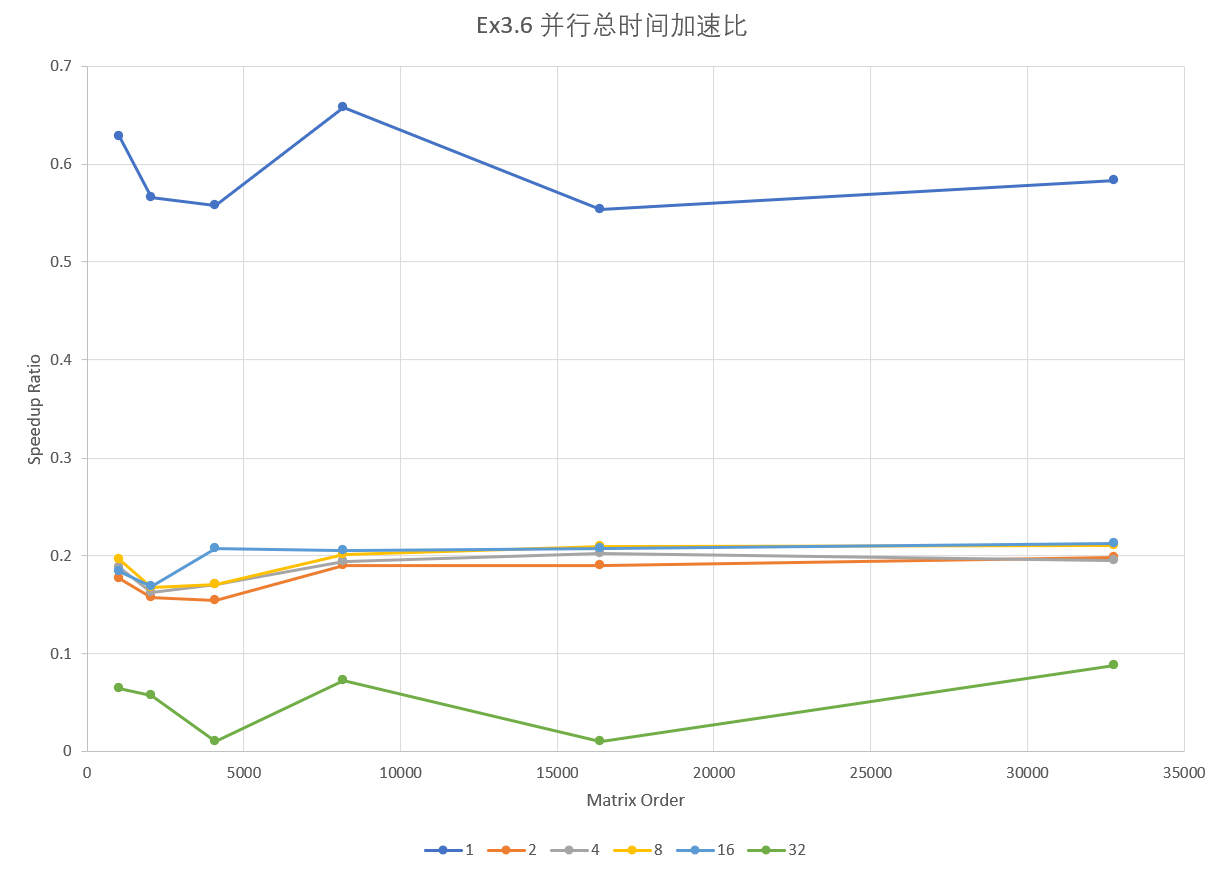
\includegraphics[width=0.85\textwidth]{35pat.png}
        \caption{Ex3.5 并行总时间加速比}
    \end{figure}
    本部分展示了并行计算时间加速比与并行总时间加速比的图表。
    由图8可以看出,并行计算时间加速比基本稳定在进程数上下,这充分体现了并行程序在计算层面的优越性。
    在这里我也思考了,为什么进程数一定时,加速比没有随着矩阵阶数明显增加。我认为这是由于进行试验时,
    最小的矩阵阶数是1024,因此最小的矩阵元素个数也有$10^8$之多,这个数量已经非常大了,因此在某一进程数下,
    计算时间加速比基本已经稳定在进程数上下。此外我们也可以注意到,当进程数达到32时,加速比随着矩阵阶数增加较为明显,这也能在一定程度上
    印证上面的说法。\\\\


    从图9中可以看出,考虑到分配时间、计算时间等时间的并行总时间加速比并不高,并且该加速比随着进程数的增加而降低,随着矩阵阶数的增加变化不明显。
    这也提醒了我们,并行程序虽然计算速度非常快,但是数据分发效率不高。这可能是由于数据的分发、汇总等都是由1个进程即0号进程进行的,这导致了效率的低下。
    一种可能的改进方法是,如果能够让多个进程同时读取到应得的数据,这样就可以大大缓解这个问题。

\clearpage





\section{Ex3.6}
\subsection{解题思路}
在本题中,我使用了附上的prog3.5\_mpi\_mat\_vect\_col.c程序完成。在这份代码中,已经基本实现了0号进程并行按列分块然后分发到不同进程的功能。
我通过修改一些参数和发送方式,完成了本题对矩阵进行分块然后再计算的要求。
我主要进行修改的地方是函数Build\_derived\_type中的MPI\_Type\_vector和MPI\_Type\_create\_resized,以及实现了通过编写不同的通信域实现最终结果的Reduce和Gather.\\\\

MPI\_Type\_vector和MPI\_Type\_create\_resized的解释已经在Ex3.5的解题思路当中详细说明了,在此不再重复。本题中
通过这两个函数的使用,成功实现了将矩阵进行分块并且发送,原理与Ex3.5相同,只不过参数进行了一些调整。与Ex3.5不同,本题
使用了Scatterv的发送方法,这是因为必须要指定发送的起始位置,才可以保证分块矩阵没有重叠地发送到各个进程中。\\\\

在编写本题时,另一个难点是如何将分块的计算结果,进行Reduce到某些核并最终Gather到0号核。在这个问题上,我参考了\url{https://mpitutorial.com/tutorials/introduction-to-groups-and-communicators/}
这篇文章中提到的方法。在Reduce时,把每一行的分块矩阵编入一个通信域,使得每行的分块矩阵Reduce到最左边的分块矩阵。在Gather时,令每一行最左边的分块矩阵Gather到0号核,即可完成计算。\\\\

下面的图10与图11示意了本题的简要流程。
\footnote{图10\url{https://pdfs.semanticscholar.org/afa8/9673d416faf99cfd6b4353ab810e8418f5d7.pdf}}
\footnote{图11\url{https://mpitutorial.com/tutorials/introduction-to-groups-and-communicators/}}

\begin{figure}[h]
    \centering
    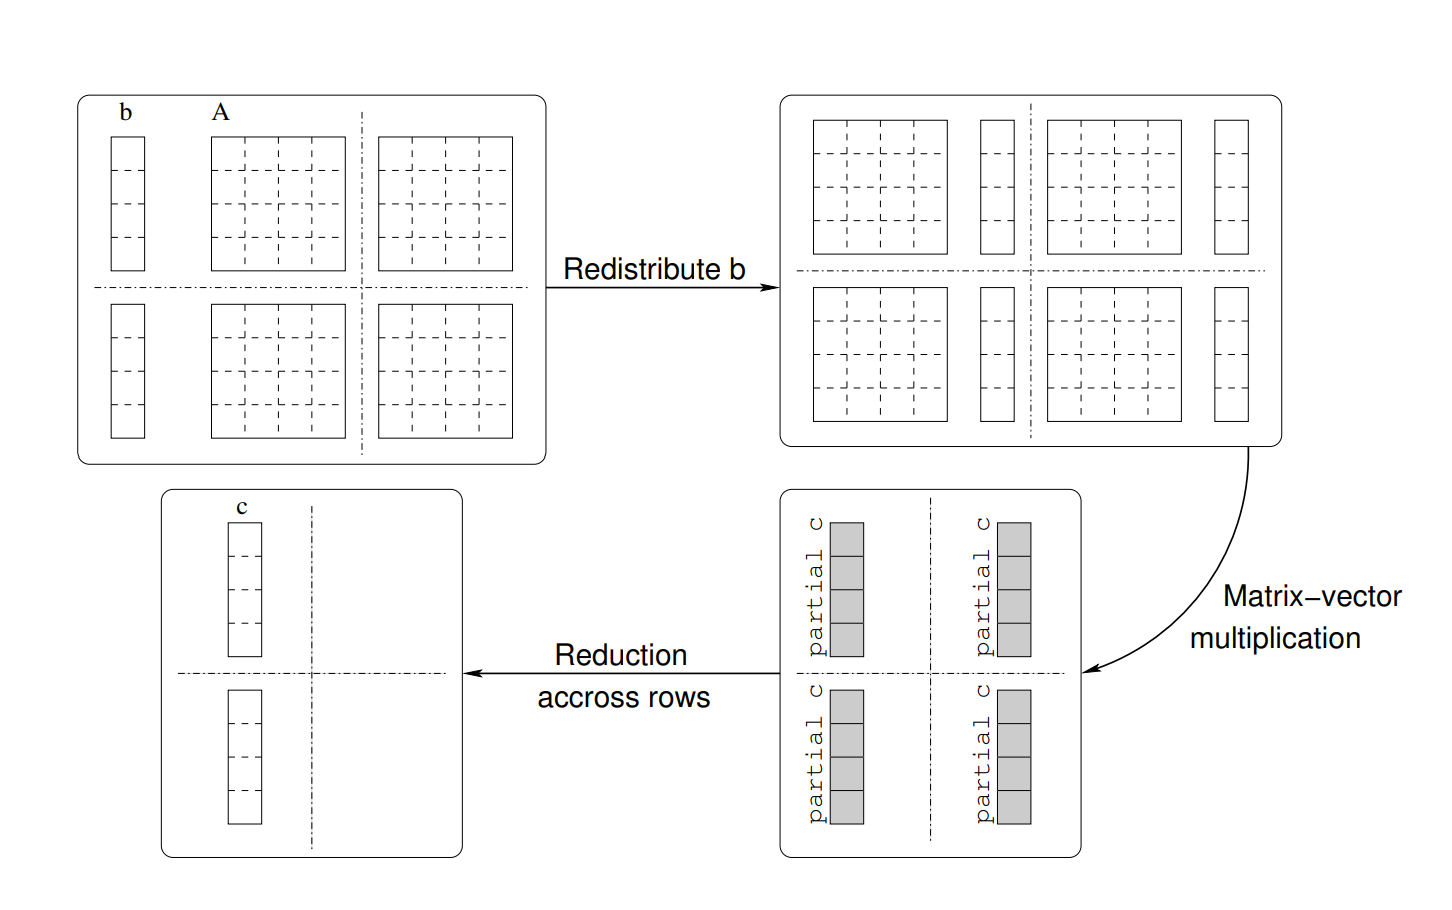
\includegraphics[width=0.7\textwidth]{cb.png}
    \caption{Ex3.6简要思路}
\end{figure}

\begin{figure}[h]
    \centering
    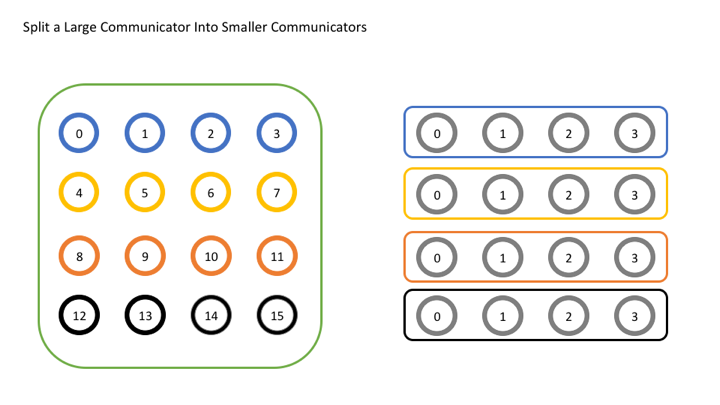
\includegraphics[width=0.7\textwidth]{comm_split.png}
    \caption{Ex3.6 Reduce时通讯子分组}
\end{figure}

\subsection{运行方式}
在集群上,只需在本题文件夹下输入make run命令即可运行本程序(makefile中设置了默认使用4进程),在运行make run后输入python check.py即可自动测试本报告中的数据,并且重定向到result文件夹下进行输出。
\clearpage


\subsection{测试结果}
本题进行的所有测试,并行计算结果与串行计算结果均相同(差的二范数为0),从而保证了并行程序的正确性。

\subsubsection{并行计算时间和串行计算时间图表分析}

\begin{table}[h]
    \caption{Ex3.6 并行计算时间 (s)}
    \label{tab:my-table}
    \centering
    \scalebox{0.8} {
    \begin{tabular}{|c|c|l|l|l|l|l|}
    \hline
    \multicolumn{1}{|l|}{}     & \multicolumn{6}{c|}{Matrix Order}                                                                                                                                  \\ \hline
    \multirow{6}{*}{Processor} & \multicolumn{1}{l|}{} & \multicolumn{1}{c|}{1080} & \multicolumn{1}{c|}{2160} & \multicolumn{1}{c|}{4320} & \multicolumn{1}{c|}{7200} & \multicolumn{1}{c|}{14400} \\ \cline{2-7} 
                               & 1                     & 0.0077                    & 0.021366                  & 0.057277                  & 0.158988                  & 0.634204                   \\ \cline{2-7} 
                               & 4                     & 0.001955                  & 0.005366                  & 0.015299                  & 0.042381                  & 0.169856                   \\ \cline{2-7} 
                               & 9                     & 0.000874                  & 0.002466                  & 0.007333                  & 0.020316                  & 0.081537                   \\ \cline{2-7} 
                               & 16                    & 0.000479                  & 0.001363                  & 0.004174                  & 0.011507                  & 0.046374                   \\ \cline{2-7} 
                               & 25                    & 0.000383                  & 0.000829                  & 0.002663                  & 0.007618                  & 0.029684                   \\ \hline
    \end{tabular}}
    \end{table}


    \begin{table}[h]
        \caption{Ex3.6 串行计算时间(s)}
        \label{tab:my-table}
        \centering
        \scalebox{0.8} {
        \begin{tabular}{|c|l|l|l|l|l|l|}
        \hline
        \multicolumn{1}{|l|}{}      & \multicolumn{6}{c|}{Matrix Order}                                                                                                               \\ \hline
        \multirow{6}{*}{Processors} &    & \multicolumn{1}{c|}{1080} & \multicolumn{1}{c|}{2160} & \multicolumn{1}{c|}{4320} & \multicolumn{1}{c|}{7200} & \multicolumn{1}{c|}{14400} \\ \cline{2-7} 
                                    & 1  & 0.0077                    & 0.021366                  & 0.057277                  & 0.158988                  & 0.634204                   \\ \cline{2-7} 
                                    & 4  & 0.001955                  & 0.005366                  & 0.015299                  & 0.042381                  & 0.169856                   \\ \cline{2-7} 
                                    & 9  & 0.000874                  & 0.002466                  & 0.007333                  & 0.020316                  & 0.081537                   \\ \cline{2-7} 
                                    & 16 & 0.000479                  & 0.001363                  & 0.004174                  & 0.011507                  & 0.046374                   \\ \cline{2-7} 
                                    & 25 & 0.000383                  & 0.000829                  & 0.002663                  & 0.007618                  & 0.029684                   \\ \hline
        \end{tabular}}
        \end{table}

        \begin{figure}[h]
            \centering
            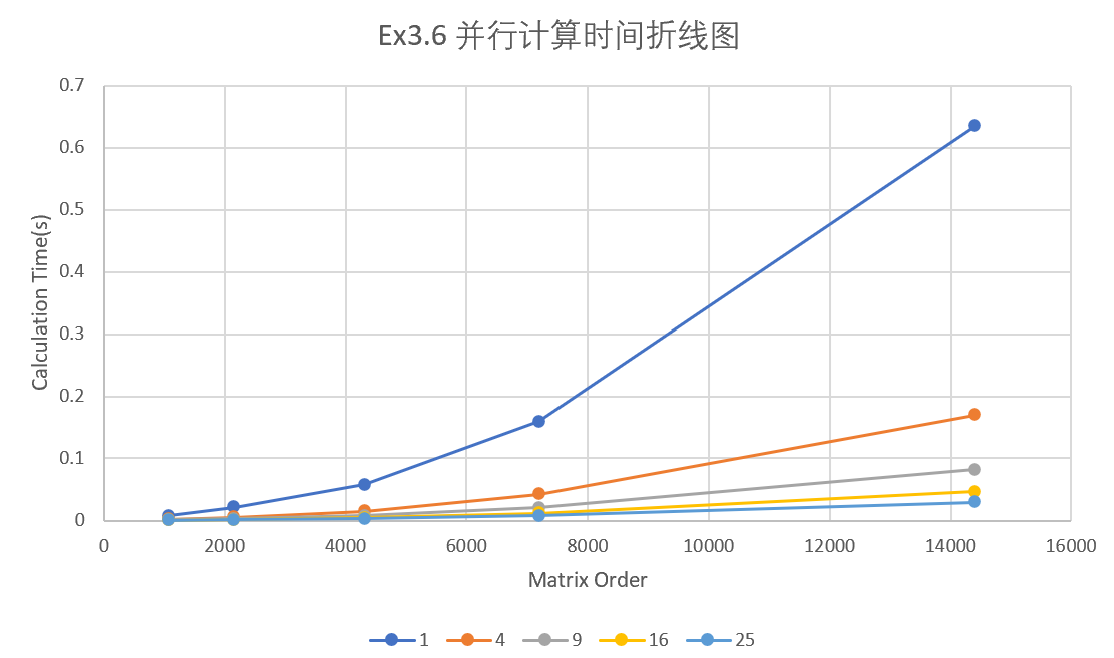
\includegraphics[width=0.85\textwidth]{36pco.png}
            \caption{Ex3.6 并行计算时间-矩阵阶数 折线图}
        \end{figure}
    
        \begin{figure}[h]
            \centering
            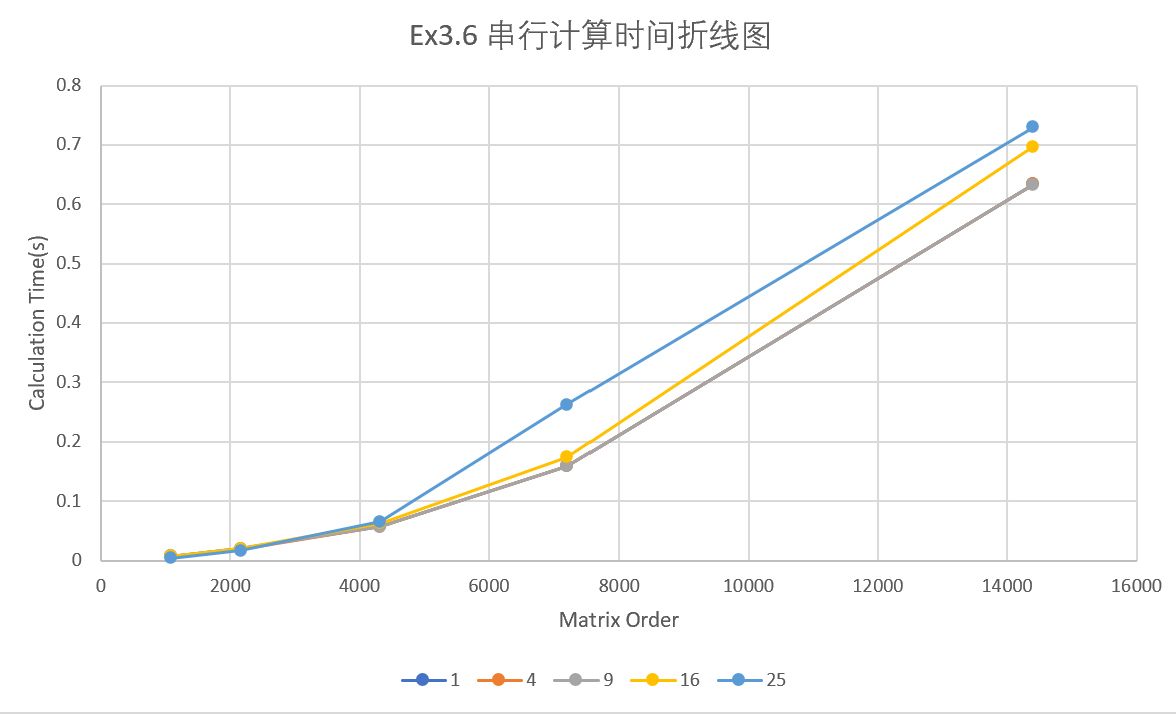
\includegraphics[width=0.85\textwidth]{36sco.png}
            \caption{Ex3.6 串行计算时间-矩阵阶数 折线图}
        \end{figure}

        本部分中展示了不同进程数下,并行和串行计算时间随着矩阵阶数的变化表格和折线图。
        从图12中可以清晰看出,与Ex3.5类似,并行计算时间与矩阵阶数成正相关。由于矩阵元素数量与矩阵阶数
        成二次关系,图中的耗时与矩阵阶数也可以近似看作二次关系。同时可以看出,进程数越多,并行计算时间越少,这也充分体现了
        并行计算在计算时的优越性。\\\\
    
        从图13中可以看出,串行计算时间与矩阵阶数近似为二次关系。不过矩阵阶数一定,不同的进程数下串行计算时间基本相同,这也基本符合串行计算
        在本实验中只由0号进程计算的事实。同时从图中和表格中都可以看到,在矩阵阶数一定时,并行计算的时间要远低于串行计算,这再一次表明了并行程序在计算方面的优越性。
    







\clearpage
\subsubsection{并行分配时间与总时间图表分析}


    \begin{table}[h]
        \caption{Ex3.6 并行分配时间(s)}
        \label{tab:my-table}
        \centering
        \scalebox{0.8} {
        \begin{tabular}{|c|c|c|c|c|c|c|}
        \hline
                                    & \multicolumn{6}{c|}{Matrix Order}            \\ \hline
        \multirow{6}{*}{Processors} &    & 1080     & 2160     & 4320     & 7200     & 14400     \\ \cline{2-7} 
                                    & 1  & 0.003992 & 0.01379  & 0.045249 & 0.127489 & 0.502016  \\ \cline{2-7} 
                                    & 4  & 0.038476 & 0.113324 & 0.324967 & 0.796448 & 3.001446  \\ \cline{2-7} 
                                    & 9  & 0.038288 & 0.116956 & 0.324326 & 0.814763 & 3.085259  \\ \cline{2-7} 
                                    & 16 & 0.039415 & 0.119221 & 0.351533 & 0.869724 & 3.335967  \\ \cline{2-7} 
                                    & 25 & 0.089289 & 0.278221 & 0.965618 & 2.596891 & 10.076753 \\ \hline
        \end{tabular}}
        \end{table}

\begin{table}[h]
    \caption{Ex3.6 并行总时间(s)}
    \label{tab:my-table}
    \centering
    \scalebox{0.8} {
    \begin{tabular}{|c|c|c|c|c|c|c|}
    \hline
                               & \multicolumn{6}{c|}{Matrix Order}                          \\ \hline
    \multirow{6}{*}{Processes} &    & 1080     & 2160     & 4320     & 7200     & 14400     \\ \cline{2-7} 
                               & 1  & 0.011692 & 0.035156 & 0.102526 & 0.286477 & 1.13622   \\ \cline{2-7} 
                               & 4  & 0.040431 & 0.11869  & 0.340266 & 0.838829 & 3.171302  \\ \cline{2-7} 
                               & 9  & 0.039162 & 0.119422 & 0.331659 & 0.835079 & 3.166796  \\ \cline{2-7} 
                               & 16 & 0.039894 & 0.120584 & 0.355707 & 0.881231 & 3.382341  \\ \cline{2-7} 
                               & 25 & 0.089672 & 0.27905  & 0.968281 & 2.604509 & 10.106437 \\ \hline
    \end{tabular}}
    \end{table}
    \begin{figure}[h]
        \centering
        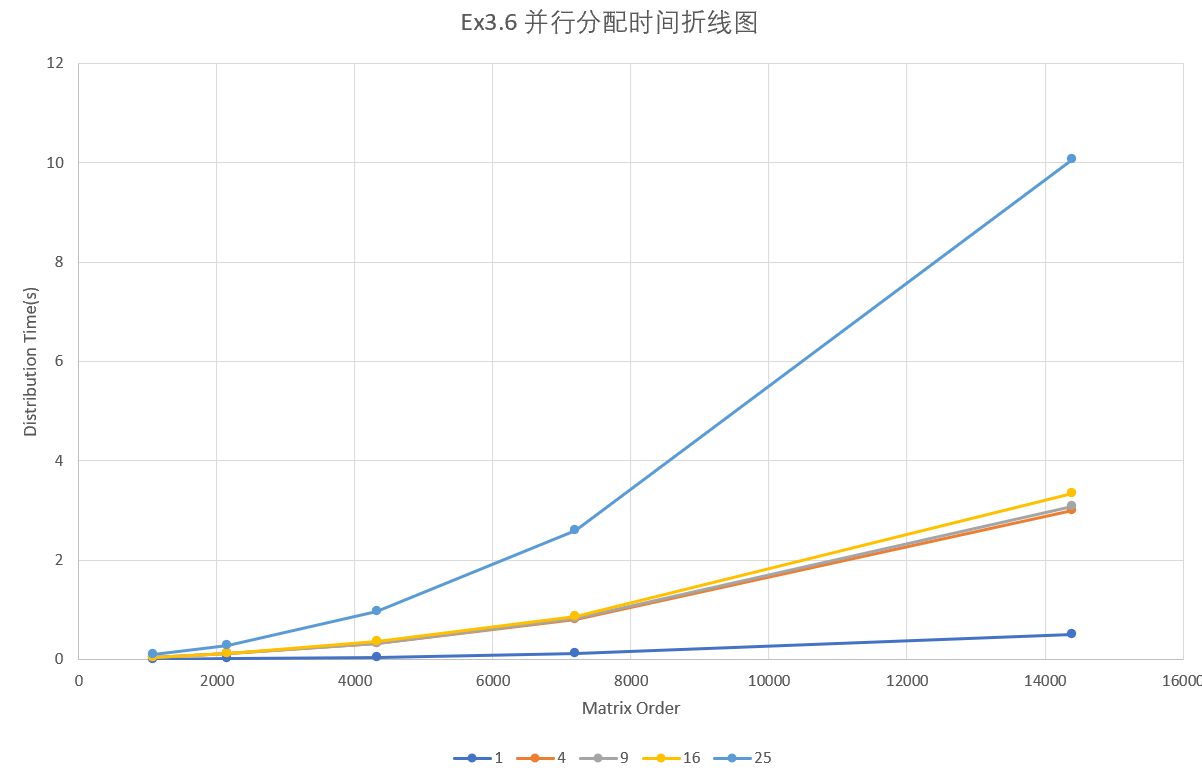
\includegraphics[width=0.85\textwidth]{36pdo.png}
        \caption{Ex3.6 并行分配时间-矩阵阶数 折线图}
    \end{figure}

    \begin{figure}[h]
        \centering
        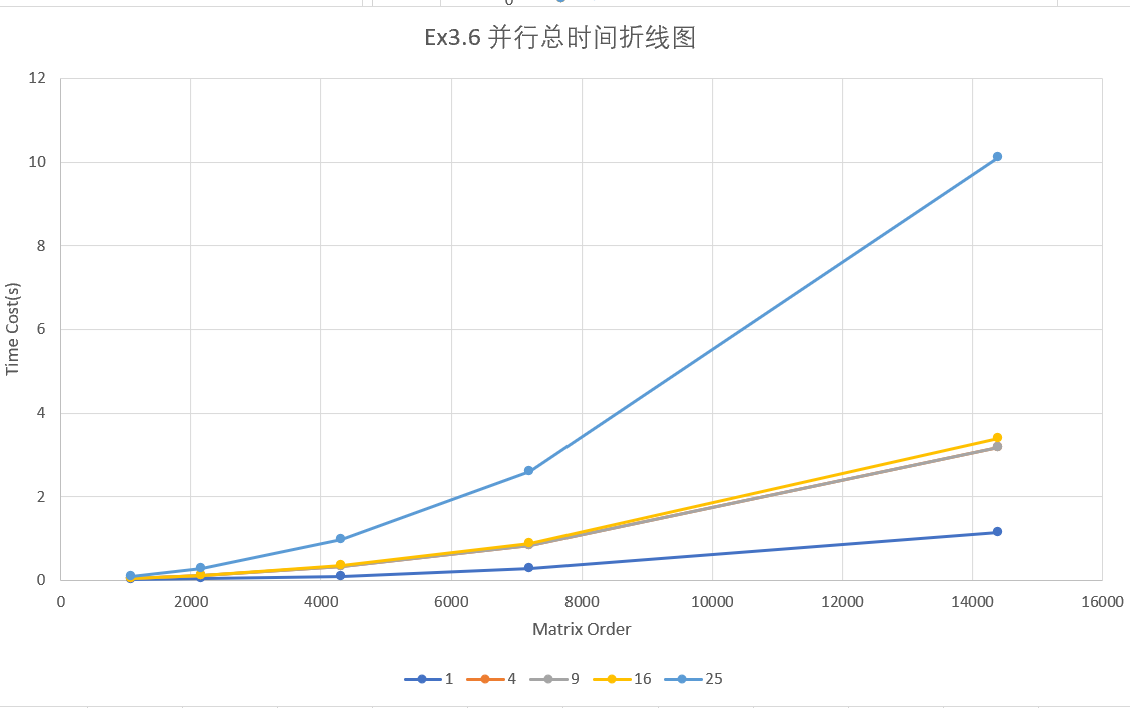
\includegraphics[width=0.85\textwidth]{36pao.png}
        \caption{Ex3.6 并行总时间-矩阵阶数 折线图}
    \end{figure}

    本部分展示了不同进程数下,并行分配时间和并行计算总时间与矩阵阶数的关系图表。
    从图14中可以看出,并行分配时间与矩阵阶数成正相关关系,
    并行分配时间可近似认为与矩阵阶数成二次关系。\\\\

    由于并行的分配时间在一定程度上远大于并行的计算时间,因此对比图14图15可以看出,并行总时间的变化趋势与并行分配时间的变化区时基本一致。

    \clearpage

\subsubsection{并行计算时间加速比与并行总时间加速比}

        \begin{table}[h]
            \caption{Ex3.6 并行计算时间加速比}
            \label{tab:my-table}
            \centering
            \scalebox{0.8} {
            \begin{tabular}{|c|c|c|c|c|c|c|}
            \hline
                                        & \multicolumn{6}{c|}{Matrix Order}                         \\ \hline
            \multirow{6}{*}{Processors} &    & 1080     & 2160     & 4320     & 7200     & 14400    \\ \cline{2-7} 
                                        & 1  & 0.947143 & 0.93382  & 1.000017 & 0.99844  & 0.999227 \\ \cline{2-7} 
                                        & 4  & 3.742711 & 3.569884 & 3.737434 & 3.741512 & 3.732085 \\ \cline{2-7} 
                                        & 9  & 8.354691 & 8.025953 & 7.798309 & 7.800354 & 7.760685 \\ \cline{2-7} 
                                        & 16 & 15.14823 & 14.42406 & 15.02827 & 15.13261 & 15.03198 \\ \cline{2-7} 
                                        & 25 & 10.62141 & 19.75513 & 24.39392 & 34.41139 & 24.59089 \\ \hline
            \end{tabular}}
            \end{table}

            \begin{table}[h]
                \caption{Ex3.6 并行总时间加速比}
                \label{tab:my-table}
                \centering
                \scalebox{0.8} {
                \begin{tabular}{|c|c|c|c|c|c|c|}
                \hline
                                            & \multicolumn{6}{c|}{Matrix Order}                         \\ \hline
                \multirow{6}{*}{Processors} &    & 1080     & 2160     & 4320     & 7200     & 14400    \\ \cline{2-7} 
                                            & 1  & 0.62376  & 0.567528 & 0.558668 & 0.554111 & 0.557739 \\ \cline{2-7} 
                                            & 4  & 0.180975 & 0.161395 & 0.168042 & 0.189036 & 0.199892 \\ \cline{2-7} 
                                            & 9  & 0.186456 & 0.165732 & 0.172421 & 0.189769 & 0.199818 \\ \cline{2-7} 
                                            & 16 & 0.181882 & 0.16304  & 0.176347 & 0.1976   & 0.206098 \\ \cline{2-7} 
                                            & 25 & 0.045365 & 0.058688 & 0.067089 & 0.100651 & 0.072227 \\ \hline
                \end{tabular}}
                \end{table}


                \begin{figure}[h]
                    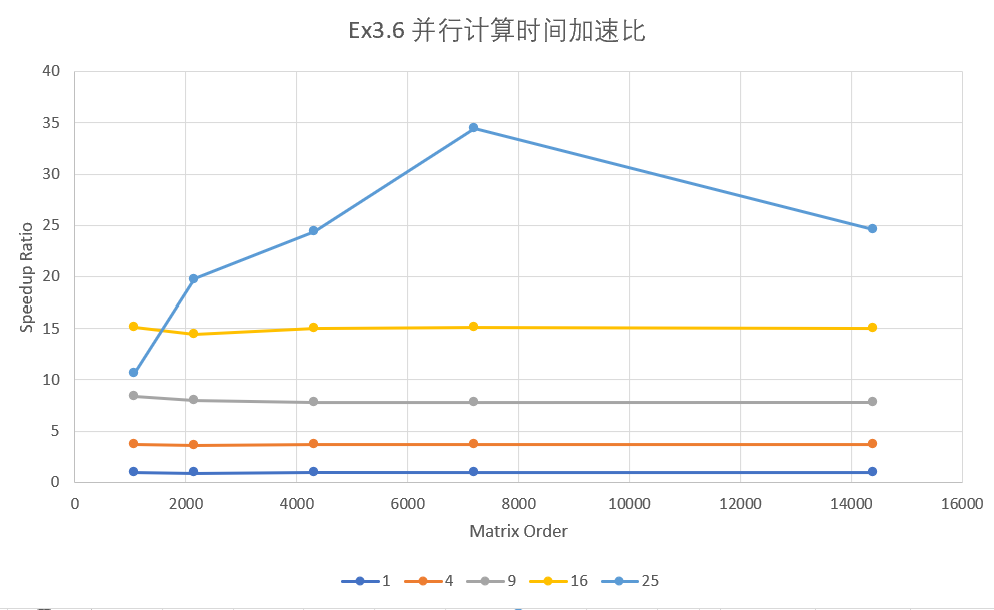
\includegraphics[width=\textwidth]{36pct.png}
                    \caption{Ex3.6 并行计算时间加速比}
                \end{figure}
                \begin{figure}[h]
                    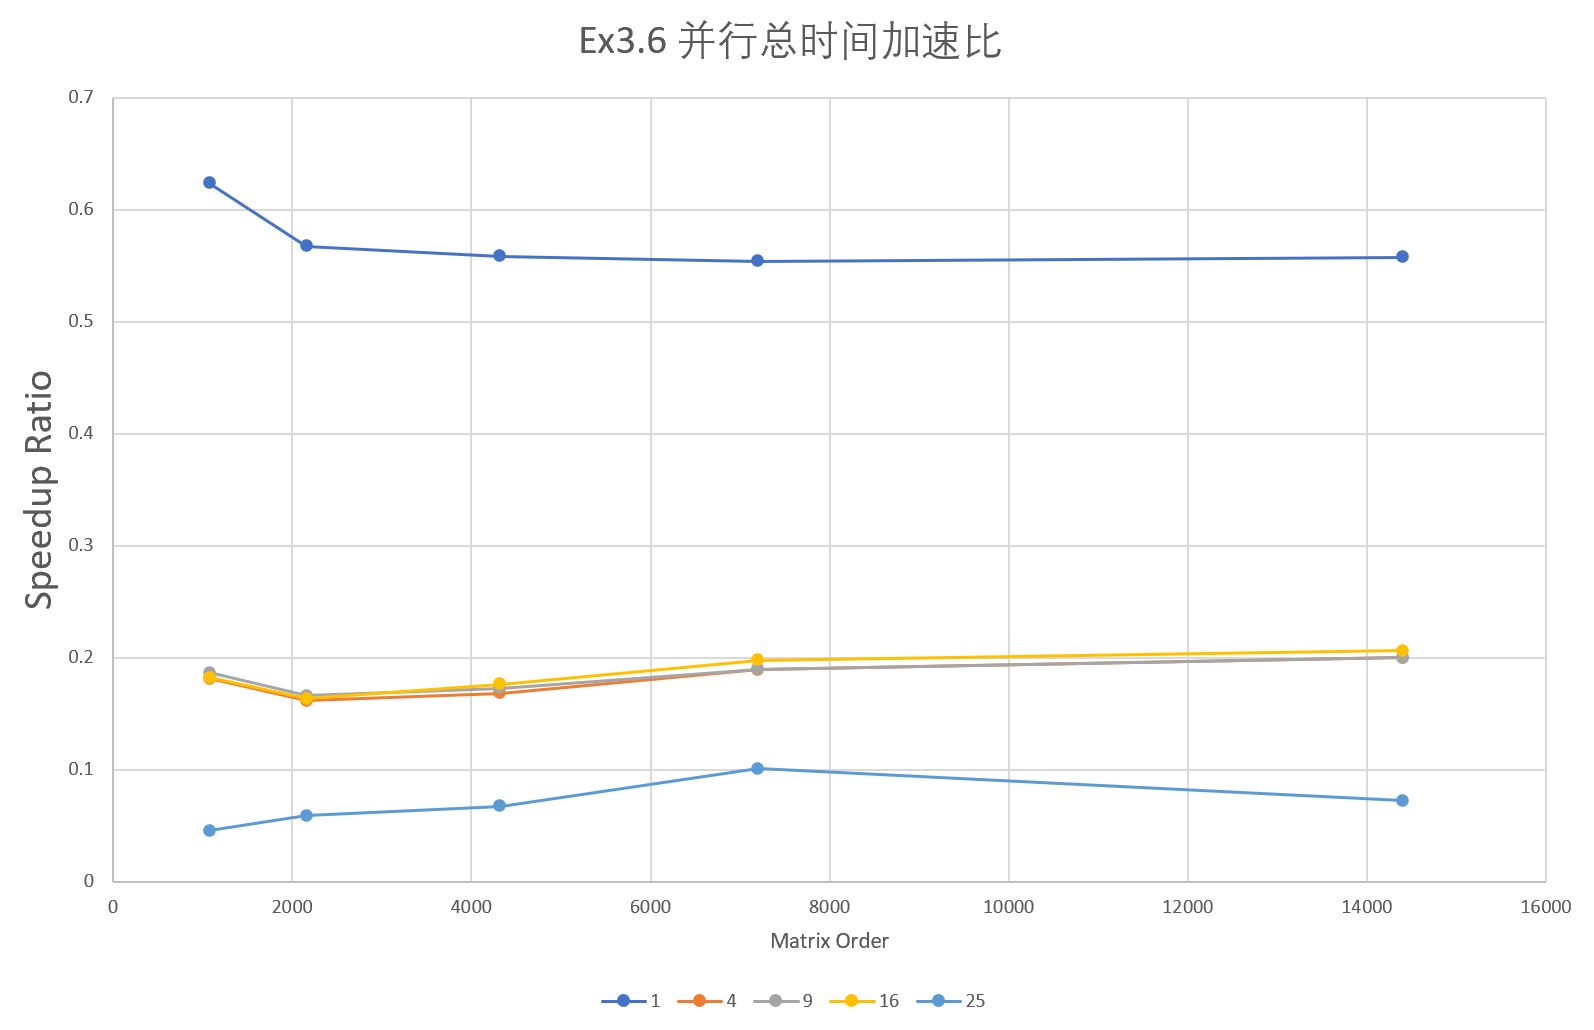
\includegraphics[width=\textwidth]{36pat.png}
                    \caption{Ex3.6 并行总时间加速比}
                \end{figure}

        本部分展示了并行计算时间加速比与并行总时间加速比的图表。
        由图16可以看出,并行计算时间加速比基本稳定在进程数上下,这充分体现了并行程序在计算层面的优越性。
        此处进程数一定时,加速比没有随着矩阵阶数明显增加的原因与Ex3.5中类似,即实验中所采用的矩阵阶数都已经较大了\\\\
        
        图16中,进程数为25时,加速比似乎有些不太正常,体现为波动较大。因此我对于进程数为25时的实验进行了额外的测试,发现的确加速比会有很大的振荡,从10-30左右的加速比均有可能出现。
        因此我认为,分块矩阵这种计算方法,可能由于计算的过程较为复杂,会产生一些波动,这也可能与OS的状态有关。\\\\
    
        从图17中可以看出,与Ex3.5类似,考虑到分配时间、计算时间等时间的并行总时间加速比并不高,并且该加速比随着进程数的增加而降低,随着矩阵阶数的增加变化不明显。
        这里与Ex3.5中得到的结论基本相同: 并行程序由于分发较为缓慢,在数据量不足够大时,效率并不一定高。

\clearpage
\section{总结}
在本次实验中,我锻炼了编写MPI并行程序的能力,也通过对运行结果的充分评估,加强了实验分析和思考的能力。
同时,我也在本次实验中锻炼了使用服务器集群的能力。\\\\
感谢老师和助教在本次实验中给予我们的悉心指导!



%----------------------------------------------------------------------------------------
%	BIBLIOGRAPHY
%----------------------------------------------------------------------------------------

\bibliographystyle{apalike}

\bibliography{sample}

%----------------------------------------------------------------------------------------


\end{document}